\documentclass[aspectratio=169,11pt]{beamer}
\usepackage[T1]{fontenc}
\usepackage{lmodern,amsmath,amssymb,booktabs,array,graphicx,tikz}
\usetikzlibrary{arrows.meta,positioning,calc}
\definecolor{navy}{HTML}{14334A}
\definecolor{teal}{HTML}{087E8B}
\definecolor{amber}{HTML}{B56317}
\definecolor{rose}{HTML}{AE3150}
\definecolor{muted}{HTML}{536571}
\setbeamercolor{normal text}{fg=navy,bg=white}
\setbeamercolor{structure}{fg=teal}
\setbeamercolor{frametitle}{fg=navy}
\setbeamercolor{alerted text}{fg=rose}
\setbeamercolor{block body}{fg=navy,bg=teal!7}
\setbeamertemplate{navigation symbols}{}
\setbeamertemplate{itemize items}[circle]
\setbeamersize{text margin left=8mm,text margin right=8mm}
\setbeamerfont{frametitle}{size=\Large,series=\bfseries}
\setbeamertemplate{frametitle}{\vspace{2mm}\insertframetitle\par\vspace{1mm}{\color{teal}\rule{\linewidth}{.65pt}}}
\setbeamertemplate{footline}{\hspace{8mm}\textcolor{muted}{\scriptsize NPS $\pi^0$ / KinC\_x60\_4b LH$_2$ / 10 September 2026}\hfill\textcolor{muted}{\scriptsize\insertframenumber}\hspace{8mm}\vspace{2mm}}
\hypersetup{colorlinks=true,urlcolor=teal,pdftitle={NPS EDTM: what is counted and what is corrected}}
\newcommand{\source}[1]{\par\vfill{\scriptsize\color{muted}#1\par}}
\newcommand{\takeaway}[1]{\begin{beamercolorbox}[sep=2.5mm,wd=\linewidth]{block body}\textbf{#1}\end{beamercolorbox}}
\newcommand{\plotframe}[3]{\begin{frame}{#1}\centering\includegraphics[width=\linewidth,height=.64\textheight,keepaspectratio]{figures/#2.pdf}\par\vspace{1mm}\raggedright\small #3\end{frame}}
\newcommand{\LE}{\widehat L_E}
\newcommand{\LF}{\widehat L_{\rm phys}}
\title{EDTM: what is counted, and what is corrected?}
\author{NPS livetime investigation}
\date{10 September 2026}
\pdfstringdefDisableCommands{\def\translate#1{#1}}
\begin{document}

\begin{frame}[plain]
\vspace{6mm}{\color{teal}\large NPS / NORMALIZATION STUDIES}\par\vspace{5mm}
{\LARGE\bfseries EDTM: what is counted,\\and what is corrected?\par}
\vspace{4mm}{\large KinC\_x60\_4b LH$_2$\quad Complete investigation update}
\vspace{5mm}\takeaway{The core estimator was already ours. The task is to match its exposure and establish its physical coverage.}
\vfill\small 43 production runs / 183 updated segments / 77,838,384 events\\
10 September 2026\quad Editable technical presentation
\par\vspace{2mm}\scriptsize No universal total-LT prescription certified. Production corrections unchanged.
\end{frame}

\begin{frame}{What is established, and what is still open?}
\begin{columns}[T]
\column{.48\textwidth}\textbf{Established}
\begin{itemize}\setlength\itemsep{3mm}
\item Same-file counting differences traced.
\item Tight timing rejects pulse-associated tags.
\item 4305 scaler deficit exists in raw data.
\item Dated EDTM route and TI4/TI6 distinction.
\end{itemize}
\column{.48\textwidth}\textbf{Still conditional}
\begin{itemize}\setlength\itemsep{3mm}
\item Detailed injection fanout and sent tap.
\item ROC5 counter-loss mechanism.
\item Pulse causality and physics weighting.
\item Final yield/charge correction and uncertainty.
\end{itemize}
\end{columns}\vspace{4mm}
\takeaway{CLT\_physics is a proposed definition, never a truth baseline or calibration target.}
\source{Current full-cache, raw, routing and source reports; complete references in the accompanying technical report.}
\end{frame}

\begin{frame}{Which data are in this edition?}
\large\begin{tabular}{@{}lrr@{}}\toprule
Population & Segments & Events\\\midrule
43 LH$_2$ production runs & 183 & 77,838,384\\
46 cached runs, including controls/junk & 187 & 79,564,296\\\bottomrule
\end{tabular}
\vspace{5mm}\normalsize
\begin{itemize}\setlength\itemsep{2mm}
\item No selected-production catalog gaps. Updated replay used consistently.
\item All 11 exact saved-file controls reproduce original NewGen counts.
\item Other saved comparisons can mix file/replay and method changes.
\item The old 168-segment presentation is historical, not this sample.
\end{itemize}
\source{Frozen manifests, file-stability checks and saved\_reproduction\_checks.csv. Five junk runs have no assigned LT.}
\end{frame}

\begin{frame}{Hall C EDTM: a probe of the path actually traversed}
\begin{columns}[T]
\column{.48\textwidth}\textbf{Intended principle}\par\vspace{2mm}
Inject artificial pulses into trigger legs, count sent pulses with scalers,
and identify recorded probes with TDC information.
\column{.48\textwidth}\textbf{The condition}\par\vspace{2mm}
The probe must traverse the stages whose loss is being corrected and sample
the relevant availability. An experiment's injection points matter.
\end{columns}
\vspace{6mm}\takeaway{EDTM does not automatically measure every detector, trigger-formation or reconstruction inefficiency.}
\source{Pooser [D01]; SHMS circulated draft [D06]. Historical descriptions are not proof of NPS wiring.}
\end{frame}

\begin{frame}{Define the stages before naming the livetimes}
\small Let $G$ be the fixed eligible physics population, $B$ formed trigger input,
$P$ prescale passage, and $R$ recorded event.
\begin{align*}
L_{\rm upstream}&=\Pr(B\mid G),\\
L_{\rm DAQ}&=\Pr(R\mid P,B,G),\\
\Pr(R\mid G)&=\Pr(B\mid G)\Pr(P\mid B,G)\Pr(R\mid P,B,G).
\end{align*}
\takeaway{With representative prescaling, $\Pr(P\mid B,G)=1/p$. The product is a conditional chain, not an independence assumption.}
\vspace{2mm}\small Threshold acceptance, readout, tracking/PID and offline selection need their own populations and no double counting.
\source{Operational definitions. A stored field called ``Computer LT'' does not specify these endpoints.}
\end{frame}

\begin{frame}{Time availability and physics survival use different weights}
\begin{columns}[T]
\column{.47\textwidth}\textbf{Time availability}
\[L_t=\frac{\int a(t)\,dt}{T}\]
A periodic pulser samples at its own pulse times.
\column{.49\textwidth}\textbf{Eligible-event availability}
\[L_r=\frac{\int r(t)a(t)\,dt}{\int r(t)\,dt}\]
High-rate periods contribute more physics events and can have more loss.
\end{columns}\vspace{5mm}
\takeaway{The same current cut helps match exposure. It does not prove identical sampling or weighting.}
\source{For stable yield per charge, $L_Q=\int I(t)L(t)dt/\int I(t)dt$. Good-helicity, yield and charge integration remains a separate requirement.}
\end{frame}

\begin{frame}{Buffering changes the relation between readout and loss}
\begin{columns}[T]
\column{.48\textwidth}\textbf{ROC lock}\par\vspace{3mm}
A readout busy can inhibit the next accept while readout proceeds.
\column{.48\textwidth}\textbf{Buffered operation}\par\vspace{3mm}
Earlier events can still be in readout when another accept is issued.
Finite queues and enabled busy sources still limit acceptance.
\end{columns}\vspace{6mm}
\takeaway{Block level 1 is one event per block. It does not prove an unbuffered whole DAQ.}
\source{Pooser [D01], Mack [D02], CODA [C04]. Logged slave broadcast buffer threshold: 5. No fixed per-event unbuffered correction adopted.}
\end{frame}

\begin{frame}{Two dated logbook entries resolve a numbering ambiguity}
\small\renewcommand{\arraystretch}{1.3}
\begin{tabular}{@{}cp{.34\linewidth}p{.49\linewidth}@{}}\toprule
No. & Local NPS TS / outgoing cable & ROC1 TI after counting-house logic\\\midrule
1 & Single cluster & One-cluster OR two-cluster OR delayed EDTM\\
2 & Cosmic scintillator & NPS cosmic OR LED\\
3 & Cosmic column OR & HMS h3/4\\
4 & Cosmic column AND & HMS hEL-REAL\\
5 & VLD & TI1 AND TI3\\
6 & At least two clusters & TI1 AND TI4\\\bottomrule
\end{tabular}\vspace{2mm}
\takeaway{Local NPS T6 is not ROC1 TI6. VTP internal decision bits are a third namespace.}
\source{\href{https://logbooks.jlab.org/entry/4170042}{4170042, 23 Aug 2023}; \href{https://logbooks.jlab.org/entry/4171556}{4171556, 29 Aug 2023}. User supplied text and confirmed applicability.}
\end{frame}

\begin{frame}{EDTM joins the NPS branch at the counting house}
\centering
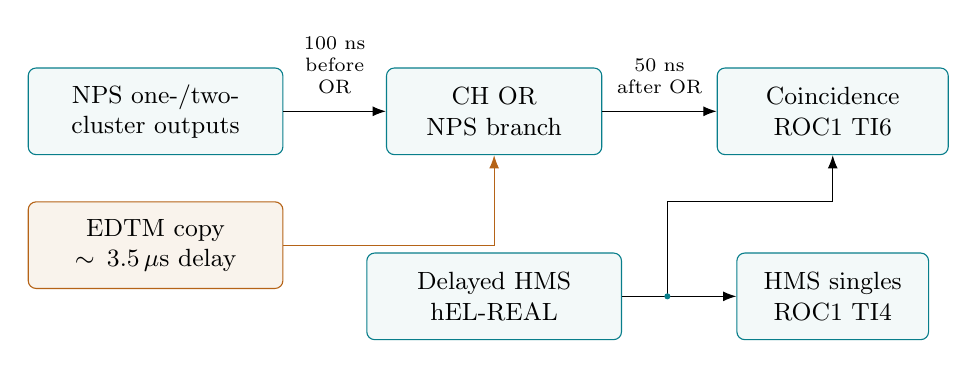
\begin{tikzpicture}[>=Latex,box/.style={draw=teal,fill=teal!5,rounded corners=1mm,align=center,font=\small,minimum height=11mm},ed/.style={box,draw=amber,fill=amber!8}]
\node[box,text width=30mm] (nps) at (0,1.35) {NPS one-/two-cluster outputs};
\node[box,text width=25mm] (or) at (4.3,1.35) {CH OR\\NPS branch};
\node[ed,text width=30mm] (e) at (0,-.35) {EDTM copy\\$\sim3.5\,\mu$s delay};
\node[box,text width=27mm] (and) at (8.6,1.35) {Coincidence\\ROC1 TI6};
\node[box,text width=30mm] (h) at (4.3,-1.0) {Delayed HMS\\hEL-REAL};
\node[box,text width=22mm] (single) at (8.6,-1.0) {HMS singles\\ROC1 TI4};
\draw[->] (nps)--node[above=1mm,font=\scriptsize,align=center,text width=12mm]{100 ns\\before OR}(or);
\draw[->,amber] (e.east)-|(or.south);
\draw[->] (or)--node[above=1mm,font=\scriptsize,align=center,text width=12mm]{50 ns\\after OR}(and);
\draw[->] (h.east)--(6.5,-1)--(6.5,.2)-|(and.south);
\draw[->] (h)--(single);
\fill[teal] (6.5,-1) circle (1.1pt);
\end{tikzpicture}
\vspace{2mm}\takeaway{The direct EDTM copy bypasses NPS cluster-trigger formation. It cannot certify losses in that bypassed chain.}
\source{Schematic from entry 4171556, not a calibrated gate diagram. HMS discriminator/EL-REAL pulser fanout and the sent-scaler tap still need detail.}
\end{frame}

\begin{frame}{The trigger cohort changes the meaning of the correction}
\begin{columns}[T]
\column{.48\textwidth}\textbf{Five TI6 runs}\par\small
4253, 4254, 4255, 4256, 4259\\
NPS branch AND HMS EL-REAL.
\vspace{3mm}\par EDTM tests an injected coincidence only if both branches receive the pulse and overlap.
\vspace{2mm}\par NPS upstream physics-trigger formation is bypassed.
\column{.48\textwidth}\textbf{38 TI4 runs}\par\small
HMS EL-REAL singles.\\
NPS cluster formation is not a requirement of that TI input.
\vspace{3mm}\par Interpret EDTM for the sampled HMS/DAQ route.
\vspace{2mm}\par NPS readout and reconstruction efficiency remain separate.
\end{columns}\vspace{4mm}
\takeaway{Do not impose a coincidence-only hardware-trigger factor on the singles population.}
\source{All 43 sole-enabled PS\_N choices and effective factors agree with the frozen summary. Working routing: entry 4171556 and user confirmation.}
\end{frame}

\begin{frame}{What we tried before, and why it did not settle LT}
\small\renewcommand{\arraystretch}{1.18}
\begin{tabular}{@{}p{.26\linewidth}p{.66\linewidth}@{}}\toprule
Earlier method & Limitation\\\midrule
Whole-file EDTM & Accepted events and sent-scaler exposure need not match.\\
Scaler L1 / input & Only tap-to-tap loss; assumes valid scaler increments.\\
TDC count times beam-on fraction & Proxy weighting, not event-by-event interval assignment.\\
EDTM-subtracted physics ratio & Same exposure issue plus pulse contribution, subtraction and sampling assumptions.\\
PRE / event-spacing / empirical repair & Require identified hardware and a validated model.\\\bottomrule
\end{tabular}\vspace{3mm}
\takeaway{Agreement among proposed definitions is not a calibration against a known truth.}
\source{Singh May 2025 [D00], inspected older code; HallC/NPS source assumptions in the report.}
\end{frame}

\begin{frame}{Preserve the actual applied NewGen reference}
\centering\includegraphics[width=.92\linewidth,height=.62\textheight,keepaspectratio]{figures/applied_NewGen.png}
\par\small Original user-supplied multipanel, unchanged. Numeric comparisons use its saved CSV and distinguish changed file coverage.
\source{The current production correction was not replaced. Old saved coverage is not the full-cache sample for every run.}
\end{frame}

\begin{frame}{The actual refinements are interval bookkeeping}
\small\renewcommand{\arraystretch}{1.45}
\begin{tabular}{@{}p{.24\linewidth}p{.33\linewidth}p{.34\linewidth}@{}}\toprule
Aspect & Original implementation & Matched diagnostic\\\midrule
Current decision & Event-stored current for E; ending TSH current for D & Same ending-interval current for E and D\\
Exposure & Event heads/tails can lack paired scaler increments & Fully covered common intervals\\
File boundaries & Denominator accumulated file by file & Join continuous segments; split gaps/restarts\\\bottomrule
\end{tabular}\vspace{4mm}
\takeaway{Unchanged: $pE/D$, prescale conversion, raw peak and broad $\pm500$ raw-channel window.}
\source{Frozen compute\_efficiencies\_stuff.cxx, prescale\_beamtime\_helper.h and diagnostic analyze.py. Not a new PID cut or complete yield/charge matching.}
\end{frame}

\begin{frame}{4398 segment0 demonstrates unsupported exposure}
\large\[\frac{19341}{19310}=1.00160539\quad\longrightarrow\quad
\frac{19292}{19310}=0.99906784\]
\normalsize\begin{itemize}\setlength\itemsep{3mm}
\item 49 EDTM tags in an unsupported tail of 1,264 recorded events.
\item Terminal scaler row changes the event boundary but repeats counters.
\item Initial cumulative counters also include exposure before the first event.
\item Later segments can restore coverage: stitch before discarding every file tail.
\end{itemize}
\source{Segment0 boundaries541321--542585. This is a local endpoint diagnosis, not the final full-run ratio.}
\end{frame}

\plotframe{4398: distinguish removal from current reassignment}{run4398_refinement_steps}{Same six files, p=1. D stays112,746; net E increases by72. The final ratio is 0.99921948. This sequence does not establish physical truth.}
\plotframe{Changes on identical files have several contributions}{method_decomposition_current}{Sequential, order-dependent shifts in percentage points. Coverage, current assignment and segment joins are not a change to the EDTM formula.}

\begin{frame}{Five counts, one prescale and a shared-count identity}
\small N=recorded; E=EDTM-tagged subset; D=sent EDTM; S=selected input; A=L1 accepts.
\[\LE=\frac{pE}{D},\qquad\widehat L_{\rm all}=\frac{pN}{S},\qquad
\LF=\frac{p(N-E)}{S-D},\qquad\widehat L_A=\frac{pA}{S}\]
\[\widehat L_{\rm all}=(1-D/S)\LF+(D/S)\LE\]
\takeaway{Accepted E is subtracted from N; sent D from S. The ratios share counts and are not independent measurements.}
\vspace{2mm}\small Physical interpretation requires verified tap/pulse correspondence, exposure and prescale sampling.
\source{Identity verified for all 43 production runs. CLT\_physics is only a proposed definition.}
\end{frame}

\plotframe{All 43 runs: ratios remain diagnostic}{refresh_livetime_comparison}{Broad raw EDTM, tight timing, pN/S and the proposed raw-subtracted ratio. Red shading marks counter defects. Values above one are retained.}

\begin{frame}{A tight timing peak does not prove complete acceptance}
\large\begin{tabular}{@{}lrr@{}}\toprule
Selection & Tags & Pulse-associated within25ticks\\\midrule
Broad raw window & 3,650,941 & 3,650,890\\
Tight corrected $\pm2$ ns & 3,650,677 & 3,650,626\\
Raw tags rejected by tight & 264 & 264\\\bottomrule
\end{tabular}\vspace{4mm}\normalsize
51 edge tags lack interpolation support. All 264 rejected tags are supported;226 pass 10 ticks.
\vspace{4mm}\takeaway{Retain the broad window as the nominal diagnostic. Tight timing is a sensitivity test, not a certified replacement.}
\source{Alternate core anchors, held-out validation; no extrapolation. Raw window is about $\pm48.83$ ns, not $\pm500$ ns.}
\end{frame}

\plotframe{Pulse phase validates association, not causal triggers}{refresh_phase_timing}{Nearby positive TDC hits can occur in a physics-triggered readout. The relative-time slope is $-3.9987366$ ns/tick for 5,515 selected points; this does not authorize counting all positive hits.}

\begin{frame}{Prescaled EDTM estimates can exceed one}
\begin{columns}[T]
\column{.48\textwidth}\textbf{Run4259: p=5}\small
\[E=6632,\quad D=32181\]
\[N=A=56200,\quad S=281210\]
\[pE/D=1.03042168\]
E/D is below one. A scaled finite sample need not be.
\column{.48\textwidth}\textbf{Conditional comparisons}\small
\[pN/S=0.99925323\]
\[p(N-E)/(S-D)=0.99522546\]
Exchangeable-label z=2.97.\\
Paired20-second block z=2.61.
\end{columns}\vspace{4mm}
\takeaway{No clipping to unity, no correction fitted to the proposed physics ratio. Sampling assumptions must be stated.}
\source{Other prescaled paired residuals below 1 sigma. Periodic probes need not satisfy exchangeability; block spread is not a hardware systematic.}
\end{frame}

\plotframe{Agreement is not a precision calibration}{refresh_correlated_difference}{Every unprescaled run is below 1.7 paired sigma, but the 35-run clean common-mean diagnostic is $(4.3734\pm1.4349)10^{-5}$ for raw; tight changes its sign. Neither ratio is a baseline.}

\plotframe{Two intervals lose almost two seconds of scaler exposure}{refresh_counter_exposure}{EDTM/clock agreement alone missed these because both counters lose exposure. Independent event timestamps expose4303/4305. No correction or production exclusion adopted.}

\plotframe{4305: the missing count is already in the raw record}{raw4305_exposure_step}{All560,647 physics fields and 660 relevant scaler snapshots agree with ROOT. L1 deficit persists through run end. Unassigned pulse-like channels are not replacement denominators.}

\plotframe{Real input-to-accept loss must remain in the livetime}{current_intervals_4398}{Near820.126s: S2082, N=A1799, D80, E69. This is a different signature from N much greater than A; do not remove real loss bursts to flatten a curve.}

\begin{frame}{TI buffering is partly established; the whole DAQ is not}
\small\renewcommand{\arraystretch}{1.35}
\begin{tabular}{@{}lp{.58\linewidth}@{}}\toprule
Logged setting & Verified interpretation\\\midrule
Firmware11.3; blocklevel 1 & Matches published TI3v11.3 label; one event/block\\
Broadcast buffer 5 & Selected threshold; local blockBuffer1 is not active\\
Busy enabled & Buffer threshold and switch-slot A/B settings\\
End Readout=Ack=L1A & Accepted counts agree with recorded totals\\\bottomrule
\end{tabular}\vspace{3mm}
\takeaway{ROC5 is distinct from npsvme5. NPS TI status and ROC end counts do not certify the scaler payload or whole-DAQ live fraction.}
\source{4303/4305 user logs; CODA header/API [C03--C04]. Current TI hardware PDF is updated 2026, so later features are not assumed for 2024.}
\end{frame}

\begin{frame}{What EDTM cannot fix by itself}
\begin{itemize}\setlength\itemsep{3mm}
\item Bypassed NPS cluster-trigger formation.
\item A sent-counter denominator with missing exposure.
\item Unidentified PRE channels or unknown injection taps.
\item Pulse association that does not identify the cause of an accept.
\item Mismatched yield, charge, helicity or trigger-population weighting.
\end{itemize}\vspace{3mm}
\takeaway{Use a stage-specific measurement and a matched population, not a plausible ratio multiplied by another plausible ratio.}
\source{Dated routing, raw-counter evidence and the conditional probability definitions.}
\end{frame}

\plotframe{Why careful livetimes matter for normalization}{refresh_normalization_sensitivity}{Lower panel holds yield and charge fixed: $L_{\rm old}/L_{\rm matched}-1$ spans $-0.76662\%$ to $+0.69107\%$. It is potential normalization sensitivity, not measured cross-section bias.}

\begin{frame}{Current decision and the remaining evidence}
\textbf{Preferred diagnostic:}\quad exposure-matched broad raw $pE/D$.
\vspace{4mm}
\begin{enumerate}\setlength\itemsep{2mm}
\item Resolve the sent tap and detailed HMS/EL-REAL injection path.
\item Obtain ROC5 readout/accumulator/FIFO source or justify matched exclusion.
\item Match physics yield, good-helicity and charge exposure.
\item Establish separate loss-stage factors only for the appropriate cohort.
\item Quantify remaining sampling and hardware-path uncertainty.
\end{enumerate}\vspace{3mm}
\takeaway{No production replacement yet. The complete report preserves the evidence, assumptions, failed alternatives and reproducible artifacts.}
\end{frame}

\appendix
\begin{frame}[plain]
\vspace{12mm}{\color{teal}\large TECHNICAL BACKUP}\par\vspace{5mm}
{\LARGE\bfseries Exact comparisons, assumptions,\\source checks and references}\par
\vspace{7mm}\large All full-cache counts retained; historical results labeled by sample.
\end{frame}

\plotframe{TI6 coincidence cohort: all five runs}{cohort_ti6}{Four runs use p=1;4259 uses p=5. Do not identify ROC1 TI6 with the local two-cluster output alone.}
\plotframe{TI4 singles: early unprescaled runs}{cohort_ti4_early}{Shading flags4303/4305. NPS hardware cluster formation is not a requirement of this configured input.}
\plotframe{TI4 singles: later unprescaled runs}{cohort_ti4_late}{Same broad/tight/proposed definitions and full-cache provenance. A near-unity value does not certify total coverage.}
\plotframe{TI4 singles: prescaled runs}{cohort_ti4_prescaled}{All five use p=2. Intentional prescaling and finite pulser sampling are separate from hardware loss.}
\plotframe{Rate plots describe associations, not a correction}{rate_comparison_by_trigger}{Selected-input rate is S divided by selected exposure. Defective scaler exposure can affect both axes. No fitted slope or empirical correction is adopted.}

\begin{frame}{Exact raw 4305 evidence and remaining cause ambiguity}
\small\begin{itemize}\setlength\itemsep{2mm}
\item File13,341,141,036 bytes; CRC32 53e8a0c0, Adler32 756ab5b0 match tape.
\item 561307 raw records,560647 physics events,660 scaler banks; complete EOF read.
\item Banks125/126:1047 events,80 tags; clock 5481 ticks, EDTM0, L1=TRIG4=2.
\item Slots6--9 advance; mapped clock/trigger group scarcely advances.
\item Later L1 minus event number stays -1046 or -1045; no recovery.
\item Slot7/ch31 and slot9/ch31 step to mapped EDTM+80; maps label them empty.
\end{itemize}\vspace{2mm}
\takeaway{Raw-record deficit established. Hardware inhibit, FIFO/accumulation/readout loss and other upstream causes are not distinguished.}
\source{One authorized raw file only. Raw 4303 was not read. No inferred missing-count repair.}
\end{frame}

\plotframe{4303: selected interval inconsistency remains flagged}{current_intervals_4303}{Events455000--456915: N1915, A=S3, E79, D1. A ratio close to one can hide cancellation elsewhere in the run.}
\plotframe{4305: selected interval inconsistency remains flagged}{current_intervals_4305}{Events105080--106127: N1047, A=S2, E80, D0. Removing an interval requires matching physics yield and charge; not done here.}
\plotframe{4551: inspect interval history, not only a run average}{current_intervals_4551}{Scaled count differences for p greater than one also contain prescale fluctuations. These plots do not assign a hardware loss to every nonzero residual.}

\begin{frame}{4350 and duplicated endpoints are different problems}
\begin{itemize}\setlength\itemsep{3mm}
\item 4350 has an updated-replay restart and near-$2^{32}$/zero-clock evidence.
\item Affected local anomalies are below the current band; components stay split.
\item Duplicate terminal rows can change event boundaries without new counts.
\item Initial cumulative exposure precedes observed event coverage.
\item A later real snapshot can legitimately span a file boundary.
\end{itemize}
\source{Frozen interval records and source behavior. Do not conflate all discontinuities or simply erase every terminal row without checking its counters.}
\end{frame}

\begin{frame}{The good-event record counters are not interchangeable}
\small\begin{tabular}{@{}lrr@{}}\toprule
4398 segment0 & TSHelH & TSH\\\midrule
Record-index range maximum & 19435 & 354\\\bottomrule
\end{tabular}\vspace{4mm}
Ranges built from TSHelH.evcount were applied to TSH.evcount in a diagnostic
gate. They do not identify the same intervals.
\vspace{3mm}\par The saved gated denominator6550 and beam time 163.950216s therefore do not represent the intended shared exposure. Main NewGen D remained19310.
\vspace{4mm}\takeaway{Use shared event/time coordinates to connect trees. Do not promote 18970/6550 to a livetime.}
\source{Original good\_event\_selection\_helper.h and prescale\_beamtime\_helper.h; documented but production code not edited.}
\end{frame}

\begin{frame}{Pulse-phase validation avoided a circular test}
\small\begin{itemize}\setlength\itemsep{3mm}
\item A20-second line fit could not track oscillator wander; replaced.
\item Alternate tight-core events anchor local interpolation; other half held out.
\item All 1,825,258 modeled held-out core events pass 25 ticks;14 fail10 ticks.
\item Per-segment99.9\% residuals:6.452--10.516 ticks. No edge extrapolation.
\item 51 nominal tags lack support; they are not claimed phase-validated.
\end{itemize}\vspace{3mm}
\takeaway{Fitted anchor residuals are not independent validation. Pulse association still does not establish trigger causality.}
\source{Full-cache phase JSON and timestamp scripts. About6,257,191.7 ticks per pulse; approximate clock agreement is not an absolute calibration.}
\end{frame}

\plotframe{All264 tight-rejected tags have pulse-phase support}{refresh_rejected_tags}{226 also pass 10 ticks. Broad-to-tight LT sensitivity reaches 0.0001595202 in 4254; it is not a complete systematic confidence interval.}

\begin{frame}{Why all-positive counting and uniform sidebands failed}
\small\begin{itemize}\setlength\itemsep{3mm}
\item 9395 positive hits lie outside the broad raw window.
\item 5515 near pulse phase track relative timing at about -4ns/tick.
\item Nearby-pulse capture in a physics readout is consistent with this pattern.
\item Among69,906,458 raw-zero events:0 within 25 ticks,2 within 50,738 within 125.
\item The phase background is not uniform around an injected pulse.
\end{itemize}\vspace{3mm}
\takeaway{Neither widening to every positive hit nor subtracting a flat phase background is justified.}
\source{Phase/timing bridge and raw-zero checks. Relative $\pm2$ns timing also fails to recover tails universally.}
\end{frame}

\begin{frame}{Uncertainty formulas have explicit sampling assumptions}
\small For independent representative pulse thinning with q=E/D:
\[\sigma(pE/D)=p\sqrt{q(1-q)/D};\quad L=1\Rightarrow\sigma=\sqrt{(p-1)/D}.\]
For exchangeable pulse labels conditional on N,S,D:
\[\mathrm E[E]=ND/S,\qquad\mathrm{Var}(E)=N(D/S)(1-D/S)\frac{S-N}{S-1}.\]
\begin{itemize}\setlength\itemsep{2mm}
\item Independent Poisson numerator/denominator errors ignore covariance.
\item Periodic pulses, beam structure and trigger overlap can violate thinning.
\item Paired blocks preserve shared-count comparisons, not unknown path systematics.
\end{itemize}
\source{Current acceptance\_tests uses paired20-second comparisons. Earlier fixed-window4398 bootstrap had its own replica count/seed; both are preserved.}
\end{frame}

\begin{frame}{TI timer registers cannot yet supply a replacement LT}
\small\begin{tabular}{@{}lll@{}}\toprule
Board0x7101150e & Initial busy & End busy\\\midrule
4303 & 0x260a & 0x1afd\\
4305 & 0x670 & 0x29a\\\bottomrule
\end{tabular}\vspace{4mm}
Initial L1A is zero but timers are nonzero; busy decreases. Latch/reset history
and common exposure have not been established.
\vspace{3mm}\par TI APIs describe timer latching and reset options. The exact online
tiStatus implementation and readout-list calls remain missing.
\vspace{4mm}\takeaway{Do not form an end-minus-start or endpoint timer ratio from these dumps.}
\source{CODA status/master-config APIs [C04c,d]. Two interleaved4305 timer chunks remain deliberately unassigned.}
\end{frame}

\begin{frame}{The event 137 parser is not a complete configuration archive}
\small\begin{itemize}\setlength\itemsep{3mm}
\item NPSlib stores text in a unique-key map using emplace: first value wins per instance.
\item Each4305 VTP config has 32 prescale entries with the same first-token key.
\item Five latency values:2560,2556,2556,2536,2536.
\item A first-key model retains only prescale ``0 1'' and latency ``2560''.
\item Original per-record/indexed raw text remains preserved.
\end{itemize}\vspace{3mm}
\takeaway{One GetInfo value is not a full multi-crate table. VTP internal prescales are not HallC TI prescales.}
\source{Inspected NPSlib source and archived raw-text model, not a reproduced pass 2 handler bug. Exact lifecycle/build not established.}
\end{frame}

\begin{frame}{ROC source discovery: useful negative results and next artifact}
\small\begin{itemize}\setlength\itemsep{3mm}
\item /u/group/nps/apps contains replay/monitoring software;2562-file bounded search archived.
\item hcana1.0.0/1.0.1/1.0.2 scaler handlers are identical offline decoders.
\item NPSlib provides timing/config/VTP clues; no ROC5 FIFO/accumulator source found.
\item Modulefiles mention /cdaqfs1/apps, unavailable on this node.
\item CODA identifies saved rol1/rol2 paths: obtain actual coin\_sparse ROC5 configuration and matching source/build.
\end{itemize}
\source{Exact commands, search scope, Git revisions, source hashes and access failures are in the evidence package.}
\end{frame}

\begin{frame}{PRE ratios require an identified input and response model}
\small\[M_w=\frac{RT}{1+Rw},\qquad r=\frac{M_{w_2}}{M_{w_1}}=\frac{1+Rw_1}{1+Rw_2}\]
\[1-L_{\rm path}\simeq\frac{\tau}{w_2-w_1}(1-r)\quad\text{at low loss}.\]
\begin{itemize}\setlength\itemsep{2mm}
\item Toy nonparalyzable Poisson monitor; same input, known widths and gating.
\item A historical 60/50 factor encodes assumptions, not a universal calibration.
\item Updating gates, recovery and coincidence logic need not follow edge losses.
\end{itemize}\vspace{3mm}
\takeaway{PRE40/100/150/200 are populated but unattributed. A40 ns pulse width does not identify PRE40. No PRE correction adopted.}
\source{Mack [D05], Crafts precedent [D07]; archived map supplies addresses, not wiring proof.}
\end{frame}

\begin{frame}{Toy models explain why a rate alone is insufficient}
\begin{columns}[T]
\column{.48\textwidth}\textbf{3-of-4 correlations}\small\par
Four independent plane availabilities0.9 give trigger survival0.9477.
\vspace{3mm}\par Perfectly shared availability0.9 gives 0.9 instead.
\column{.48\textwidth}\textbf{Event-spacing model}\small
\[f(\Delta t)=R e^{-R(\Delta t-\tau)},\quad\Delta t\ge\tau\]
\[L=1/(1+R\tau)\]
Requires stationary Poisson input and fixed nonparalyzable dead interval.
\end{columns}\vspace{5mm}
\takeaway{Buffering, burst structure and correlations can invalidate these models. Neither is fitted as an NPS correction here.}
\source{Mack [D02,D05]; operational toy examples. Minimum event spacing alone is not total live fraction.}
\end{frame}

\begin{frame}{Historical NPS repairs and slopes stay historical}
\small\begin{itemize}\setlength\itemsep{3mm}
\item March 2024 workflow: raw-time peak, I greater than 2 uA, pulser-scaler repair and terminal-readout removal.
\item Later local DT\_Analyzer\_new.C adds an inferred missing-scaler contribution.
\item July 2024 KinC row:19 runs, maximum TRIG1 rate1200 kHz, slope entry -2.13 under literal header $10^{-5}$ \%/kHz.
\item Original fit units, sample and cause need verification; no slope correction adopted.
\end{itemize}\vspace{3mm}
\takeaway{A previous convention or resolved task does not certify a different replay and exposure.}
\source{Zhang [N02,N04,N05,N06]; local source snapshot provenance retained.}
\end{frame}

\begin{frame}{Earlier four formulas, explicitly}
\small H0: whole-file selected-trigger TDC; F0: raw-EDTM-zero subset;
E0: positive raw EDTM. Current-selected scalers carry subscript c.
\[f_A=A_c/A_0,\quad f_D=D_c/D_0\]
\begin{align*}
L_{\rm EDTM,old}&=pE_0/(D_c/f_D)=pE_0/D_0,&L_{\rm TSH,old}&=pA_c/S_c,\\
L_{\rm TDC,old}&=pH_0f_A/S_c,&L_{\rm phys,old}&=pF_0f_A/(S_c-D_c).
\end{align*}
\takeaway{Beam-on fractions are proxies. The EDTM simplification requires a valid nonzero unclipped fraction.}
\source{Inspected older compute\_luminosity\_scaler.cxx; Singh May 2025 [D00]. These formulas are not the current common-interval definitions.}
\end{frame}

\begin{frame}{Stored LT fields are not interchangeable}
\small\begin{tabular}{@{}lrl@{}}\toprule
4398 record & Value & Scope\\\midrule
Older database CPU\_LT & 0.9992 & Rounded component,2-uA condition\\
Fixed-window study, I greater than 2 uA & 0.99920687 & Proposed physics component\\
Master Computer\_live\_time & 0.992 & Different unresolved provenance\\
Same-cache original NewGen & 0.99858088 & Current original method\\
Matched broad raw & 0.99921948 & Exposure-matched diagnostic\\\bottomrule
\end{tabular}\vspace{4mm}
\takeaway{Matching rounded values supports at most component consistency, not total-loss coverage.}
\source{Older active nps\_livetimes.h reads CPU\_LT; its previous calculator is commented out.}
\end{frame}

\foreach \part in {1,...,5}{
\begin{frame}{Production ratios: table \part\ of 5}
\centering\small\input{sections/slide_table_\part.tex}
\par\vspace{3mm}\raggedright\small Old and raw use the same refreshed files. Tight is diagnostic. Flag ! means counter-exposure inconsistency. Full counts and proposed ratios are in the report/CSV.
\end{frame}}

\begin{frame}{Source guide: Hall C principles and the user's work}
\small\begin{itemize}\setlength\itemsep{3mm}
\item \href{https://indico.jlab.org/event/946/contributions/16510/attachments/12602/20074/Luminosity_nps_collaboration_meeting_2025.pdf}{Singh May 2025 [D00]}: earlier definitions and luminosity context.
\item \href{https://hallcweb.jlab.org/DocDB/0010/001022/001/pooser_live_time.pdf}{Pooser, DocDB1022 [D01]}: HallC EDTM and DAQ formalism.
\item \href{https://hallcweb.jlab.org/DocDB/0010/001001/002/EDTMnonPoissonBiasCorrectionv2.pdf}{Mack, DocDB1001 [D02]}: unbuffered periodic-pulser conditions.
\item \href{https://hallcweb.jlab.org/DocDB/0011/001110/002/DetailedDeadtimeSourcesv2.pdf}{Mack, DocDB1110 [D05a]}: leading edges, updating and recovery.
\item \href{https://hallcweb.jlab.org/DocDB/0010/001063/002/Combinatorics\%20in\%20Estimating\%20the\%20Hodo\%203of4\%20Trigger\%20Livetimev2.pdf}{Mack, DocDB1063 [D05b]}: plane/trigger correlations.
\end{itemize}\source{Original PDFs and manifests packaged. Other-experiment conditions are not imported as NPS hardware facts.}
\end{frame}

\begin{frame}{Source guide: NPS and timing studies}
\small\begin{itemize}\setlength\itemsep{3mm}
\item \href{https://redmine.jlab.org/attachments/download/1499/EDTM_Study_Report.pdf}{Murphy, PionLT2022 [N01]}: tails and multi-trigger sampling.
\item \href{https://indico.jlab.org/event/866/contributions/14914/subcontributions/234/attachments/11505/17805/NPS_July17_2024_Raydo.pdf}{Raydo, July 2024 [N03]}: NPS trigger/readout distinction and embedded config.
\item \href{https://redmine.jlab.org/issues/837}{Zhang NPS chronology [N04--N06]}: February/March timing and scaler studies.
\item \href{https://indico.jlab.org/event/866/contributions/14918/subcontributions/283/attachments/11529/17843/Deadtime\%20and\%20Efficiency.pdf}{Zhang, July 2024 [N02]}: prior LT/rate comparisons; units remain qualified.
\item Crafts May 2025 [D07], SHMS draft [D06], archived run plan and trigger layouts: supporting context.
\end{itemize}\source{Full titles, URLs, pages, scope and local files are in REFERENCES.md and the report appendix.}
\end{frame}

\begin{frame}{Source guide: actual routing, logs and CODA}
\small\begin{itemize}\setlength\itemsep{3mm}
\item \href{https://logbooks.jlab.org/entry/4170042}{4170042,23 Aug 2023 [L01]}: local NPS outputs and firmware capabilities.
\item \href{https://logbooks.jlab.org/entry/4171556}{4171556,29 Aug 2023 [L02]}: counting-house timing, EDTM OR and ROC1 map.
\item User logs4303/4305 [L03,L04]: saved originals, exact endpoint/register checks.
\item \href{https://coda.jlab.org/drupal/}{CODA portal [C00--C08]}: TI3v11.3 masks/APIs, ROL configuration and version-qualified manuals.
\item Local NPSlib/hcana/replay source and raw comparison: exact hashes and search histories in evidence.
\end{itemize}\source{Logbook text/dates provided by user, applicability confirmed; web expired-auth error prevented independent retrieval of L01/L02 pages.}
\end{frame}

\begin{frame}{Edit and reproduce without rerunning ROOT}
\small\begin{itemize}\setlength\itemsep{3mm}
\item Edit presentation.tex for these slides; report.tex and sections/report\_body.tex for the technical report.
\item Run bash build.sh to build both PDFs. It does not regenerate or overwrite prose sources.
\item REPORT.md is the parallel narrative; generate\_report.py deliberately regenerates the article body/tables only when requested.
\item make\_comparisons.py regenerates new plots from frozen summaries/intervals.
\item Verify SHA256SUMS before edits; keep an edited copy if preserving the issued version.
\end{itemize}\takeaway{Full counts, references, source snapshots, commands and uncertainty limitations are supplied for independent review.}
\source{ROOT/raw reproduction instructions are retained separately. No additional staging or production job is needed to edit these documents.}
\end{frame}
\end{document}
